\section{Experiments}   \label{sec:experiments}
% Experiments

We evaluate the model-based position control approach proposed in section \ref{sec:technical-approach} by applying it to a real system composed of FREE actuators in parallel, and measuring the error in tracking a set of desired end effector states. 

%In order to evaluate the model-based position control approach proposed in section \ref{sec:technical-approach}, we use our model to compute the pressure inputs needed to achieve a set of end effector positions, then measure the error 

%% Description of system identification
Our model requires experimental system identification of the elastomer force, $\f_\tx{elast}$, from \eqref{eq:pequation}. This is done by measuring the end effector position $\x'$ over a random sampling of control pressures $\p'$, calculating $\f_\tx{elast}' = - \left( \J_{\x}^T (\x') \p' + \f_\tx{load} \right)$ at each point, then approximating $\f_\tx{elast} (\x)$ as 2nd degree polynomial of $\x$ using least-squares regression.

%% Summary of experimental procedure
We approximate the workspace of the system via the process explained in section \ref{sec:technical-approach}. We then define a set of desired end effector states within the computed workspace and solve \eqref{eq:QP} to find suitable pressure inputs to achieve each one. We measure the actual state of the system under these input pressures, and compare the measured states to the desired ones. We quantitatively characterize the performance of our model-based control strategy with both the root-mean-square error and maximum error over all points tested. Preliminary results of this kind are presented in section \ref{sec:results}.


%% figure: the 2dof and 3dof modules, labeled, side to side
\begin{figure}
    \centering
    \begin{tikzpicture}
        \def\colWidth{0.4\linewidth}
        \matrix [row sep=0.5cm, column sep=1cm, style={align=center}] (my matrix) at (0,0)
        {
        \node[style={anchor=center}] {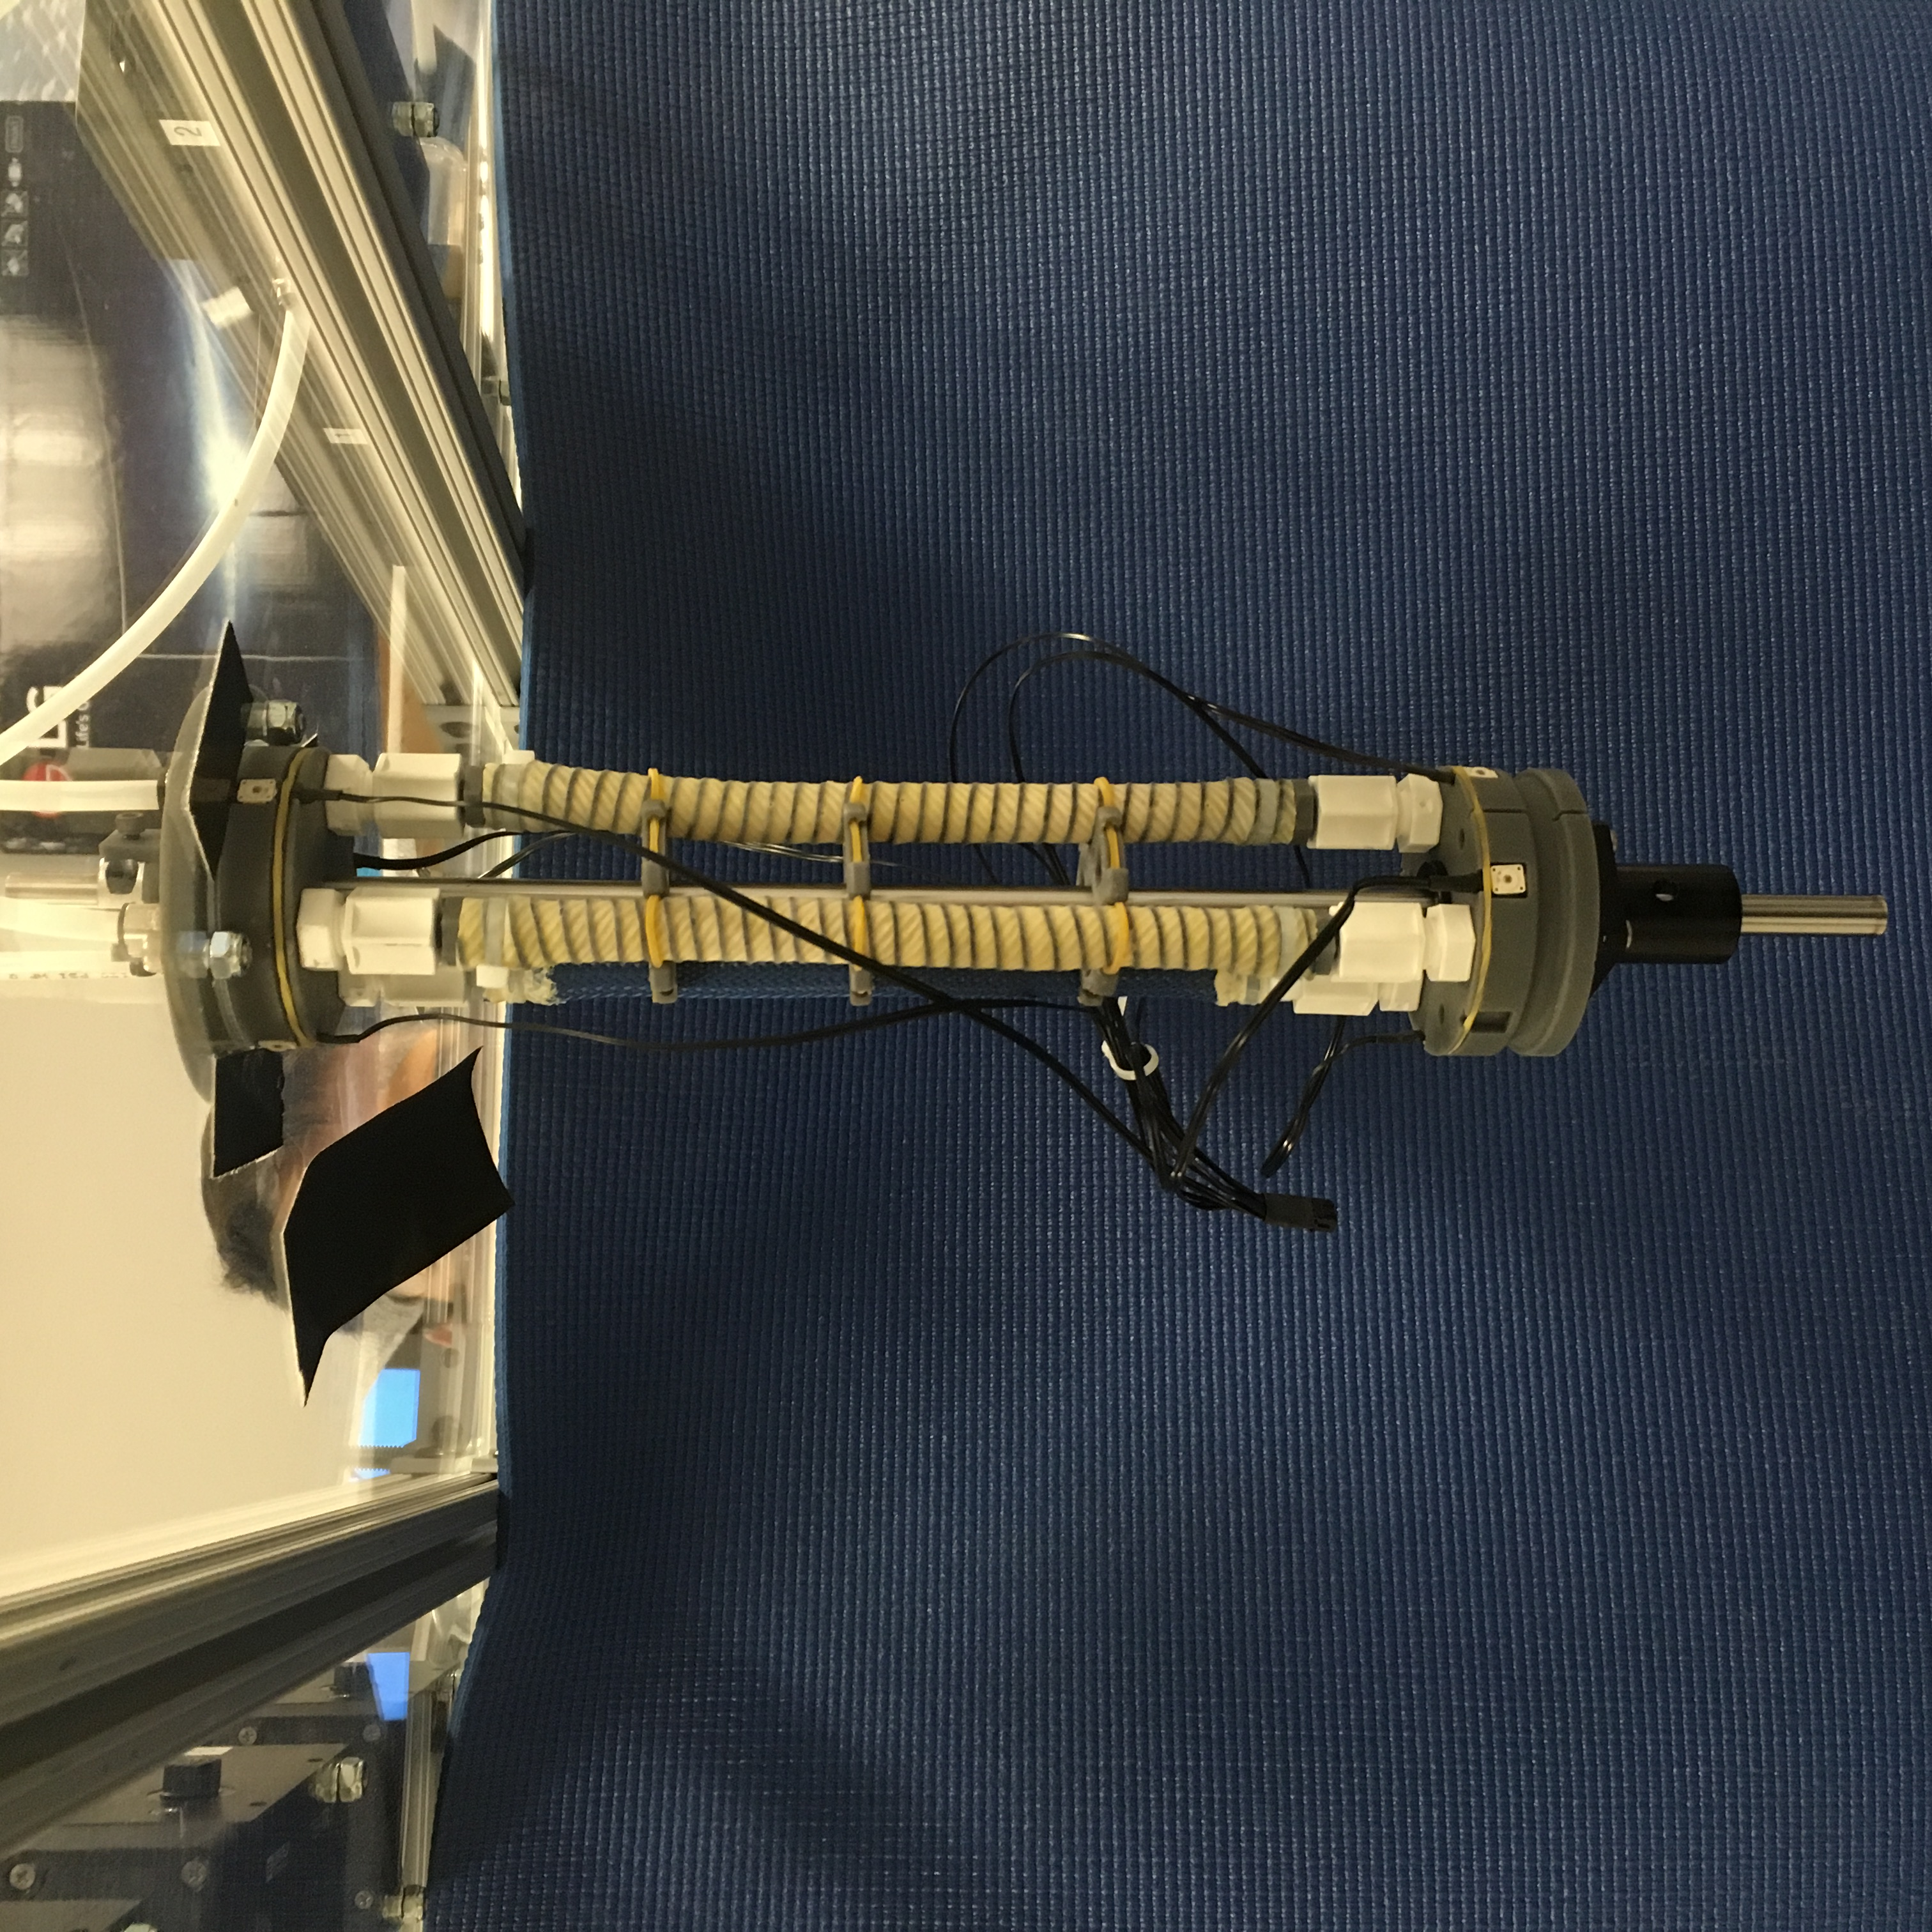
\includegraphics[width=\colWidth, angle=-90]{figures/free3.JPG}};
        &
        \node[style={anchor=center}] {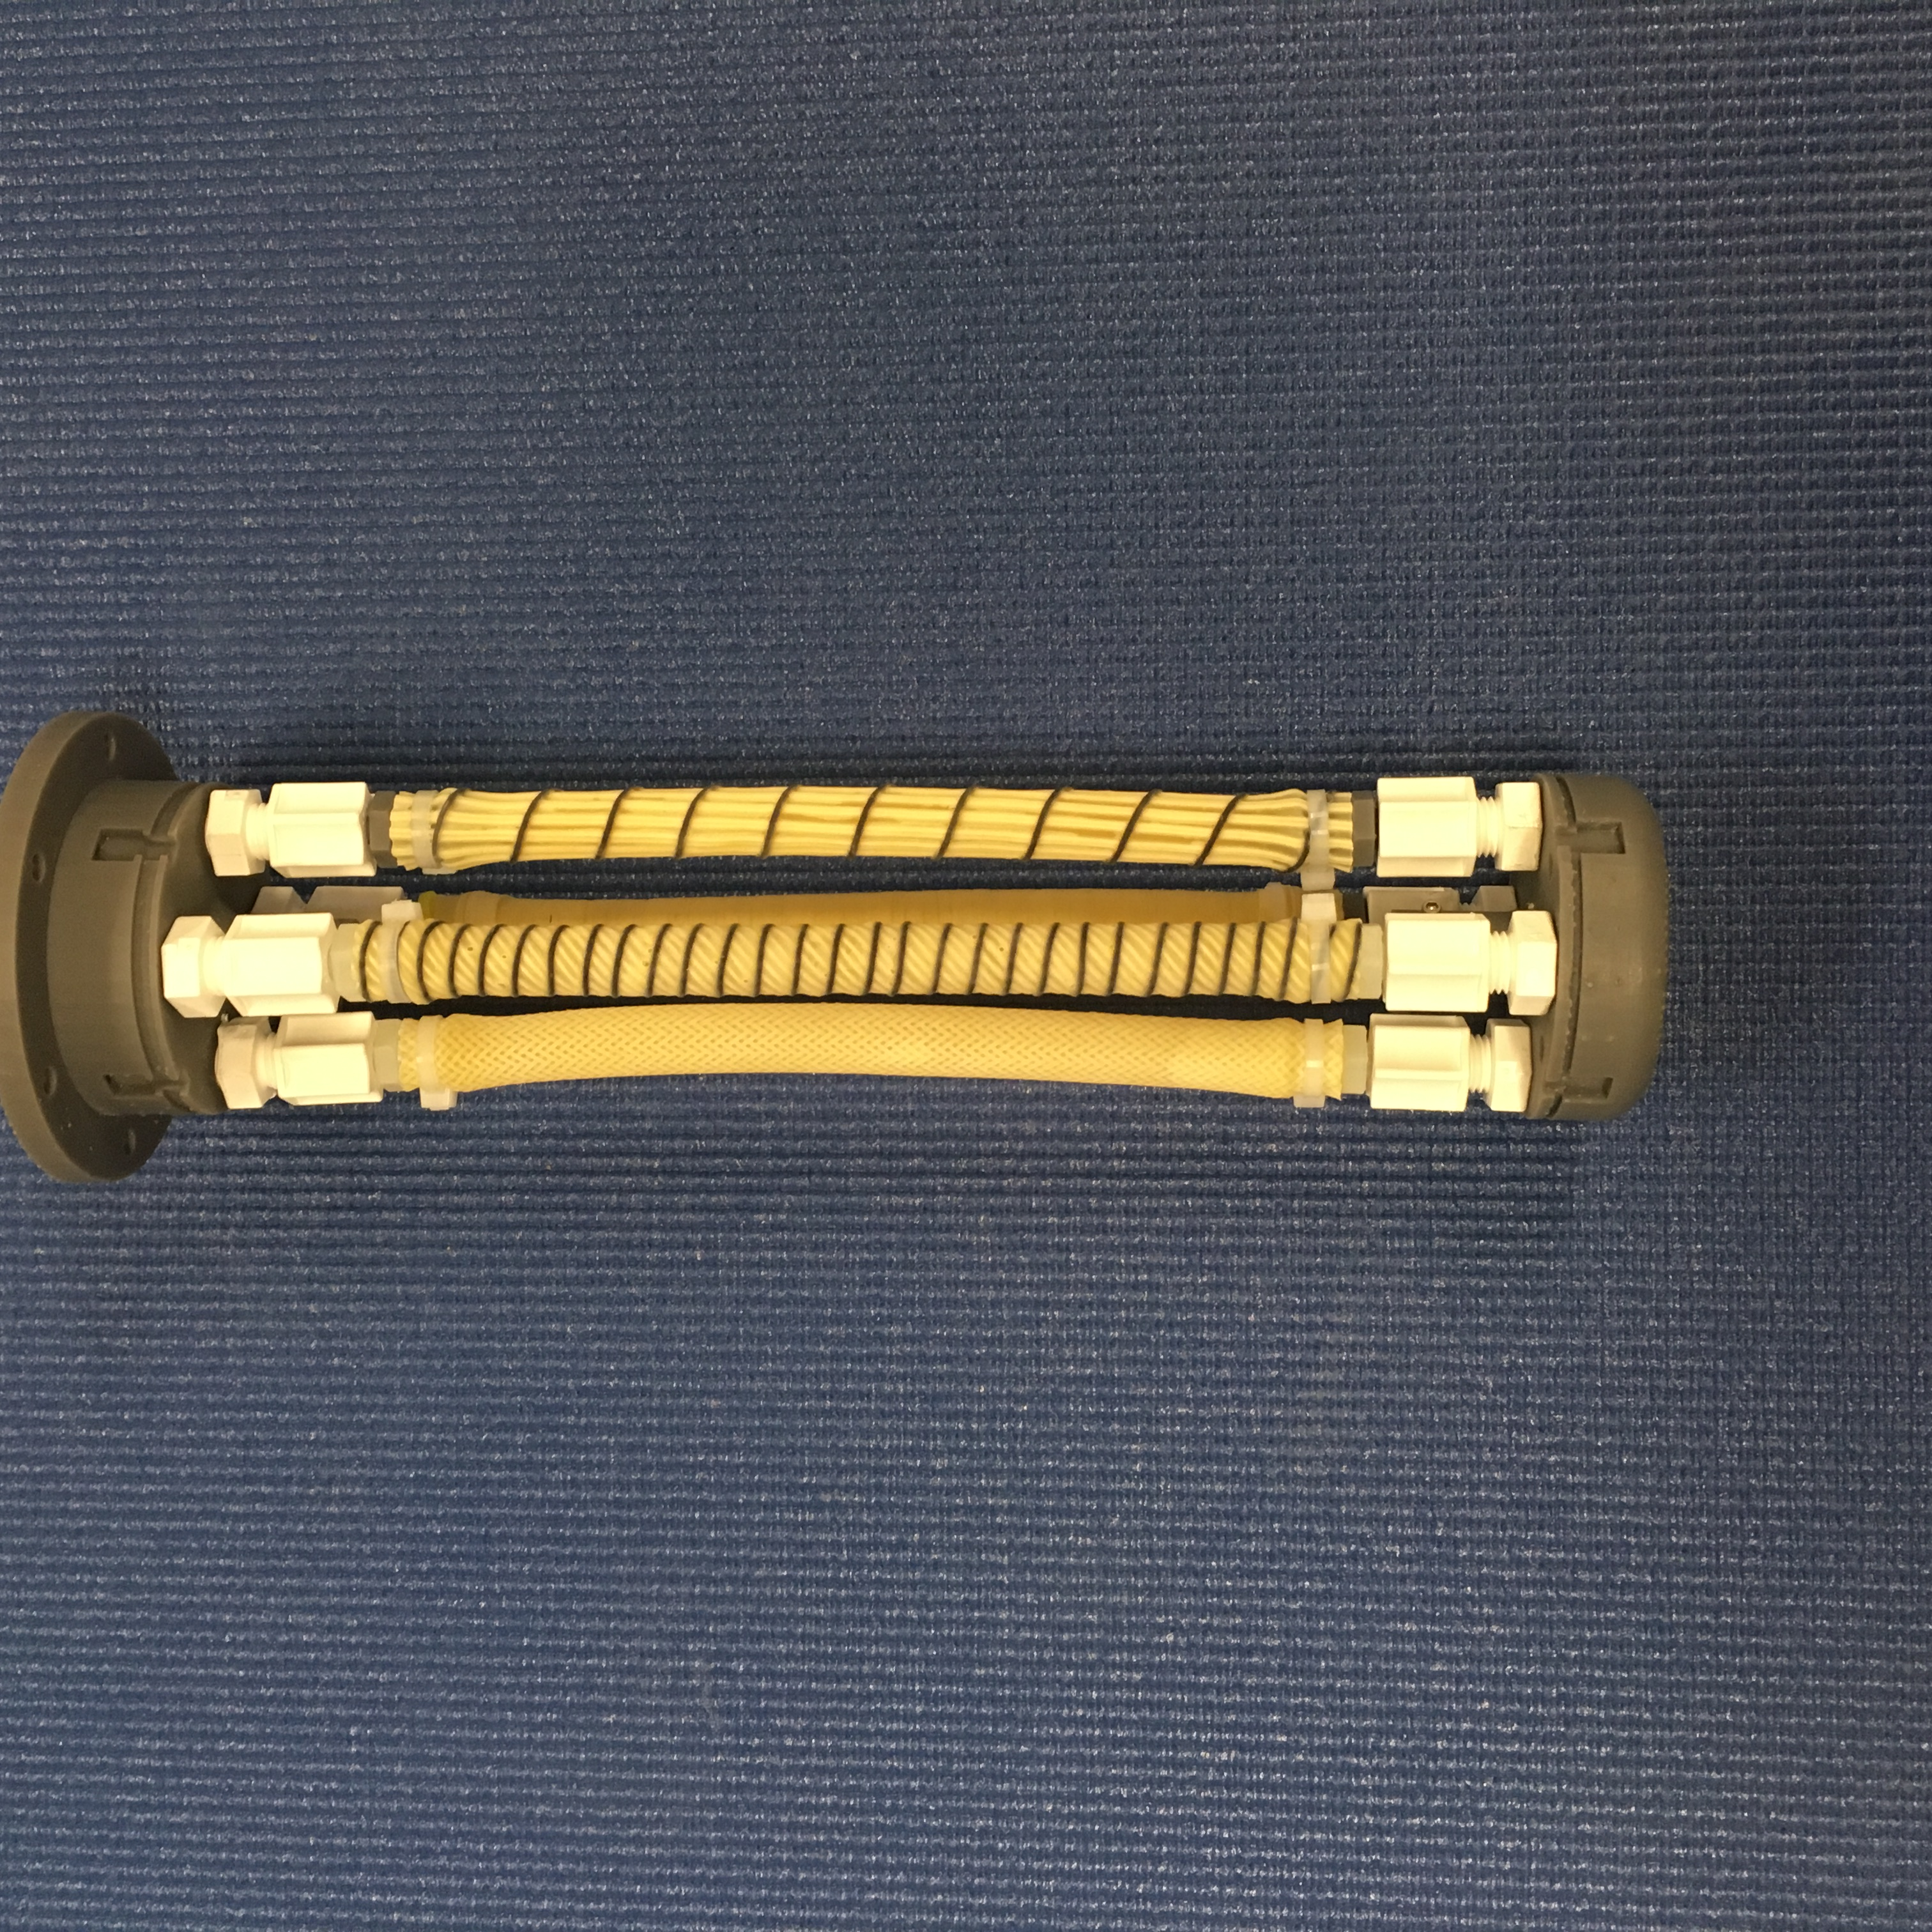
\includegraphics[width=\colWidth, angle=-90]{figures/free4.JPG}};
        \\
        };
    \end{tikzpicture}
    \caption{(a) A parallel system consisting of three FREE actuators attached to an end effector that is constrained to 2 DOF motion. A linear/rotary ball bearing allows the end effector to translate and rotate about a central shaft, while restricting motion in all other directions. (b) A parallel system consisting of four FREE actuators attached to an end effector that is constrained to 3 DOF motion. A centrally mounted spring-steel shaft  constrains the end effector to move on a 2D sub-manifold of 3D space, while also admitting rotations about its central axis. \Dan{these pictures/captions are placeholders. Will be replaced with much nicer versions with labels drawn on to show DOFs.}}
    \label{fig:modules}
\end{figure}

%% Equipment used in experiments
We conduct experiments on two parallel soft actuator systems. The first consists of three actuators constrained to 2 DOF motion (Figure \ref{fig:modules}a). The second consists of four actuators constrained 3 DOF motion (Figure \ref{fig:modules}b). So far, all of our experiments have been conducted using the three actuator system. In future experiments, we will apply the same model-based control approach to the less constrained system shown in figure \ref{fig:modules}b. During the experiments, the pressures inside the actuators are varied using pneumatic pressure regulars (Enfield TR-010-g10-s), and the displacement of the end effector is measured using a motion capture system (Phase Space Impulse X2E).
